\documentclass[aps,prl,twocolumn,groupedaddress]{revtex4-1}
%\documentclass[11pt]{amsart}
%\usepackage{geometry}                % See geometry.pdf to learn the layout options. There are lots.
%\geometry{letterpaper}                   % ... or a4paper or a5paper or ... 
%\usepackage[parfill]{parskip}    % Activate to begin paragraphs with an empty line rather than an indent
\usepackage{graphicx}
\usepackage{amsmath}
%\usepackage{amssymb}
%\usepackage{epstopdf}
%\DeclareGraphicsRule{.tif}{png}{.png}{`convert #1 `dirname #1`/`basename #1 .tif`.png}
\begin{document}

\title{Improving Dark Matter Axion Searches with Active Resonators}
\author{G. Rybka, A. Malagon, L. McBride, K. Patel}
\email[]{grybka@uw.edu}
\affiliation{University of Washington}
\date{}                                           % Activate to display a given date or no date

%runnning list of figures we need in the paper:
%plot of snr vs Q for signal sent in on resonance; with and without delay line
%plot of snr vs Q for a measurement made one peak away from tallest peak
%plot of S_11 with and without delay line
%plot of snr vs Q for the new delay line in the transition region
% all of the above needs to be done with the new couplings as we changed the coupling coefficients
% after shipping the demo delay line back. Ask Lisa what those coupling coefficients are.
% perhaps change the coupling coefficients and see where the sweet spot is for snr improvement?
%

\date{\today}

%copied directly from Gray's original arxiv paper
\begin{abstract}
Axions are a well motivated candidate for dark matter.  The most sensitive experiments searching for dark matter axions rely on the coupling of axions to the electromagnetic resonances of a microwave cavity immersed in a strong magnetic field.  The sensitivity of the experiment is proportional to the $Q$ of the resonance that is coupled to axions.
To date, the resonators used in axion searches have all been passive, with $Q$s limited by power loss in the cavity walls.  I propose the use of active feedback resonators to increase the $Q$ of microwave cavity axion dark matter experiments by several orders of magnitude.
This should allow experiments to significantly increase the rate at which they can test potential axion masses and couplings.
%this is too bold a claim; realistically we can only get to 10^6 before signal power plateaus.
\end{abstract}

\pacs{}

\maketitle

\section{Introduction} 
%copied directly from Gray's original arxiv paper.

The axion is a hypothetical particle that is both a candidate for dark matter and a result of the Peccei-Quinn solution to the strong CP problem~\cite{Peccei,Peccei_2,PhysRevLett.40.223,PhysRevLett.40.279,Preskill1983127,Abbott1983,ipser-sikivie}.
Axions with masses below $10^{-3}$ eV are particularly interesting because they could be produced in sufficient quantities to account for 
%cold
dark matter~\cite{Turner199067}.
For axions in this mass range the coupling between axions and photons
%say two photon coupling?
, despite being exceptionally weak, provides the best chance of directly observing axion dark matter.

The most sensitive dark matter axion searches to date have been of the ``microwave cavity" type.
%somehow the assumption that axions form all of the dark matter halo is lost...
These experiments rely on the conversion of axions from the local dark matter halo into photons in a strong magnetic field.
This conversion is resonantly enhanced when the resonant frequency of the microwave cavity is equal to the frequency of the photons produced from the axion conversion~\cite{PhysRevLett.51.1415}.
%again, the missing information is that axions are non-relativistic, better way to say it is that the energy deposited into the electromagnetic field excites a resonant mode of the cavity. this might be a good time to bring in the energy dispersion.
Operation of these experiments involves slowly tuning the resonant frequency of the microwave cavity to explore different potential axion masses and searching for an excess of power deposited from dark matter axion conversion.
Microwave cavity experiments have been demonstrated to have the sensitivity required to detect optimistically coupled dark matter axions over a small mass range,
%maybe say explicitly from 2-4 microeV
but as of yet, axions have not been detected in a microwave cavity experiment~\cite{PhysRevLett.104.041301}.

The signal power in microwave cavity experiments is proportional to a number of factors, including the local density of dark matter, the strength of the magnetic field, the volume of the cavity, and the resonant 
%loaded
quality factor $Q$ of the resonance being used:
%give equation
\begin{align}
P_{sig} = \eta g_{a\gamma\gamma}^2B_{ext}^2VC\frac{\rho_a}{m_a}\text{min}(Q_{loaded},Q_a)
\end{align}
The primary background is the thermal noise from the physical temperature of the cavity and the electronic noise from the first stage amplifier.  
The figure of merit for a microwave cavity experiment is the instantaneous axion signal to noise ratio (SNR).
%why emphasize instanteneous?
The SNR is given by the ratio of the signal power to the fluctuations in the noise power. We assume that we measure the signal for time $\tau$ with a frequency resolution equal to the width of the axion signal, $B_a$:
\begin{align}
SNR = \frac{P_{sig}}{\delta P_{noise}} = \frac{P_{sig}}{T_{noise}B_a}\sqrt{B_a \tau}
\end{align}

Experiments with a larger SNR can be sensitive to more pessimistic axion photon couplings for a given frequency tuning speed or tune more quickly for a given axion photon coupling sensitivity.

Increasing the cavity $Q$ is one way to increase SNR in a microwave cavity experiment; the speed at which the cavity frequency can be tuned while remaining sensitive to a given axion photon coupling is linearly proportional to $Q$~\cite{Peng2000569}.
The presence of a strong magnetic field precludes the use of high-$Q$ superconducting cavities in these experiments, so the cavities are usually made of or coated with copper.
%add, ``...although R&D is being done with superconducting thing films on the walls...''
Loaded $Q$s of $10^5$ at 1 GHz have been achieved with copper cavities in axion experiments~\cite{Peng2000569}.  Higher frequency cavities typically have smaller $Q$s.
%mention anomalous skin depth limit, or scaling of Q with frequency as f^-2/3?
%The quality factor for a passive resonator depends solely on the frequency, geometry, and material of the resonator.
For a cylindrical copper cavity the Q scales as $Q \propto f^{-2/3}$....skin depth.

I present here a means of artificially increasing the $Q$ of the cavity resonance using active feedback in order to improve sensitivity to dark matter axions and increase the speed at which different axion masses can be tested.

\section{Theory of Method}

\begin{figure}
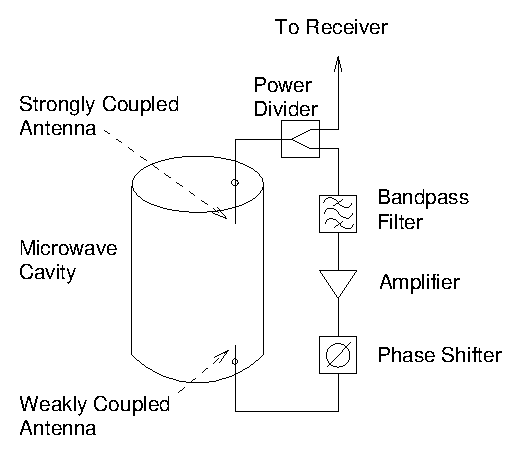
\includegraphics[width=7cm]{figs/experiment_schematic.eps}
\caption{\label{fig:experiment_schematic} Schematic of active feedback resonator for an axion experiment}
\end{figure}

\begin{figure}
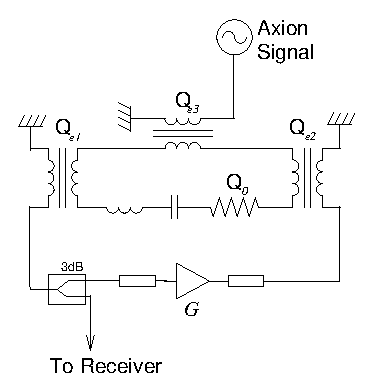
\includegraphics[width=6cm]{figs/equivalent_circuit.eps}
\caption{\label{fig:equiv_circuit} Equivalent circuit to axion photon conversion in microwave cavity with active regeneration}
\end{figure}

\begin{figure}
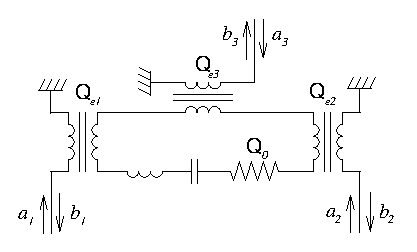
\includegraphics[width=6cm]{figs/amplitude_definitions.eps}
\caption{\label{fig:amplitude_defs} Microwave cavity represented as three port device.}
\end{figure}

The use of active feedback resonators is a well established technique used in regenerative receivers~\cite{armstrong1914wireless}.
It involves connecting positive feedback to a resonator at the appropriate phase and amplification such that the power lost each oscillation to the output and damping effects is nearly completely replaced.  
This has the effect of increasing the $Q$ of the system.
%perhaps say here that it will also amplify the noise of the system. However we show that the SNR improves square-rootishly with multiplier.
A schematic of a microwave cavity axion experiment with active feedback is shown in Fig.~\ref{fig:experiment_schematic}.   Power from axion to photon conversion exits the cavity via a strongly coupled antenna, some of which is sent to a detector.  The remainder of the power is amplified, phase shifted, and then fed back into the cavity via a weakly coupled antenna.  A filter may also be needed to select the desired mode. 

%We can derive the increase in Q and noise using an equivalent circuit model of the cavity and feedback system.
%We represent the cavity as an RLC circuit, with impedance transformers representing the coupling ports from the cavity to the external system.
%An amplifier with voltage gain $\sqrt{G_a}$ and equivalent noise temperature $T_a$ is placed in the feedback loop along with a phase shifter.
%The closed loop gain of the system, assuming no loss in the phase shifter, is then $\sqrt{G_l} = S_{12}\sqrt{G}$. When 
To calculate the effect of the active feedback, I will use the equivalent circuit to the cavity-amplifier system shown in Fig.~\ref{fig:equiv_circuit}.  The cavity resonant mode is equivalent to an $LRC$ circuit with an unloaded $Q$ of $Q_0$ and the coupled antennas are equivalent to transformers with couplings $Q_{e1}$ and $Q_{e2}~$\cite{Montgomery:1948}.  These external quality factors can be defined in terms of the unloaded Q and the coupling coefficients $\beta_1$ and $\beta_2$, which represent respectively the fraction of power lost out of port 1 or port 2 compared to the power lost to the walls: $Q_{e1} = Q_0/\beta_1$ and $Q_{e2} = Q_0/\beta_2$. $G$ is the combined gain of the amplifier and power divider.  There is also a phase shift between the two antennas around the loop, which will be denoted as $\delta$.  The coupling between the electromagnetic resonance in the cavity and dark matter axions is equivalent to a third antenna with coupling $Q_{e3}$.  The passive loaded $Q$ of the resonator is $Q_L=\left(Q_0^{-1}+Q_{e1}^{-1}+Q_{e2}^{-1}+Q_{e3}^{-1}\right)^{-1}$.

The cavity is fully characterized by the scattering matrix S and the noise amplitudes $c_1$ and $c_2$ radiated by the cavity into cold matched loads. Element $S_{21}$ is equal to the voltage amplification factor.

Let us look at the amplitude of the wave at the output of port 2, assuming that all components are impedance matched and that isolators are placed at the ports to prevent reflected waves. If port 2 is critically coupled, then the noise wave at its output is equal to $c_2^2 =kT_{cav}B$, where B is the bandwidth of the detector.(G is the voltage gain of the amplifier and $n_a$ the noise wave associated with it.) We can add the noise of the cavity and the amplifier to get the system noise wave, $n(t) = c_2(t)+n_a(t)$.

The time averaged noise power of the output is then
\begin{equation}
P_n = \langle |n(t) + n(t-t_1)GS_{21} + (c_2(t-2t_1)+n_a(t-2t_1))G^2S_{21}^2 + \ldots|^2 \rangle
\end{equation}
The amplifier noise $n_a$ and the thermal noise from the cavity $c_2$ are independent, hence $<c_2n_a> = 0$, and also in the steady state $<c_2(t)>^2 = \bar{c_2}$ is independent of time, so

\begin{equation}
P_n = (\bar{c}_2^2 + \bar{n}_a^2)\frac{1}{1 - G^2|S_{21}|^2} + \text{cross-terms} \\
\end{equation}
where the cross-terms hold the information about the coherence of the noise between feedback rounds. Any signal entering the cavity undergoes exponential decay, so the expectation value of the cross terms goes as $<(c_2(t-nt_1)c_2(t-mt_1)> = \bar{c_2}^2e^(-(|n-m|)t_1/\tau)$, where $\tau = Q_L/\omega_0$ is the coherence time of the cavity. One can see that when the roundtrip time around the feedback loop is much larger than the coherence time, $t_1 \gg \tau$, the cross terms are exponentially suppressed and the feedback loop and amplifier enhance the original noise temperature of the cavity by a factor:
\begin{equation}
T_n = T_{sys}\frac{1}{1-G^2|S_{21}|^2}
\end{equation}

The analysis is slightly different for the signal power. We treat the axion-converted signal as a continuous source with amplitude $e_a$. Then the signal power observed at the output of port 2 (with the feedback loop is
\begin{equation}
P_s = \langle |e_a(t) + e_a(t-t_1)GS_{21} + e_a(t-2t_1)G^2S_{21}^2 + \ldots|^2 \rangle
\end{equation}

and as long as $\omega t_1$ is a multiple of $2\pi$, $e_a(t-nt_1) = e_a(t)$.

Therefore the time averaged signal power is
\begin{equation}
P_s = \bar{e}_a^2\frac{1}{(1 - GS_{21})^2}
\end{equation}

This implies that the enhanced SNR from the feedback loop will be greater than the passive SNR, $SNR_0$, (assuming the same integration time and axion bandwidth) in the limit where the roundtrip time is much longer than the coherence time of the cavity, (need to add extra factor because axion signal will additionally be enhanced by Q).

\begin{align}
\frac{SNR_{e}}{SNR_{0}} &=\frac{P_{s, enhanced}}{P_{s,original}}\frac{T_o}{T_e} = \frac{Q_e}{Q_o}\frac{1-G^2|S_{21}|^2}{(1-GS_{21})^2} 
\\ &= \frac{1}{1-GS_{21}}\bigg(1 + \frac{2GS_{21}}{1-GS_{21}}\bigg)
\end{align}
In most cases we can achieve loaded Q's of only an order of magnitude below the axion linewidth, so we need a combined feedback of $GS_{21} = .8$ to improve the Q by an order of magnitude.

When $t_1 \approx \tau$ we can no longer ignore the cross terms and end up with a noise power of

\begin{equation}
P_n = (\bar{c}_2^2 + \bar{n}_a^2)\frac{1}{1 - G^2|S_{21}|^2}\frac{1}{1-2e^{-t/\tau}GS_{21}}
\end{equation}

One subtlety is that if there is only phase shifter for multiple frequencies within the feedback loop, one will not be able to hold the requirement that $\omega t = 2\pi$ when the roundtrip travel time $t$ is long; that is to say, interference fringes will begin to be observed within the bandwidth of the cavity when tis of the order $t \approx \pi Q_e / \omega_0$, so in order to avoid this effect, one would want a delay which longer than the coherence time of the cavity, but not too long so as to avoid deconstructive interference among frequencies slightly off resonance. Another solution would be to multiplex the signal and give each frequency a slightly different phase shift so that all the frequencies in the cavity bandwidth receive a 2$\pi$ phase shift around the loop.

The SNR will plateau once we can no longer assume that the signal persists indefinitely - that is to say, when we include the $Q$ of the signal in our description of the signal power, we get that the
As well, the enhanced Q (again assuming a phase shift of $2\pi$), is given by \cite{ref:frenchpaper}
\begin{equation}
Q_e = Q_L\frac{1}{1-GS_{21}}
\end{equation}
you can see this by noting that the Q is a measure of how much a signal builds up; since the signal builds up by 
$Q_{unloaded} = \omega U / P_{walls}$.
Similarly
$Q_{e1} = \omega U / P_{port1}$ and $Q_{e2} = \omega U / P_{port2}$.
Therefore the loaded passive Q is $Q_L^{-1} = P_{total lost}/\omega U =  = Q_{e1}^{-1} + Q_{e2}^{-2} + Q_{unloaded}^{-1}$.
Then with the feedback loop some power is regained, so 
$Q_e^{-1} = 1/\omega U (P_{port1} + P_{port2} + P_{walls} - P_{feedback}) = Q_L$
%% I can now treat the cavity as a three port device using amplitudes defined in Fig.~\ref{fig:amplitude_defs} with an $S$ matrix of
%% \begin{equation}
%% S = \left( \begin{array}{ccc}
%%   -1 + 2 \beta_1 (1 + \beta_1 + \beta_2)^{-1} & 2\sqrt{\beta_1\beta_2}(1 + \beta_1 + \beta_2)^{-1} \\
%%   2\sqrt{\beta_1\beta_2}(1 + \beta_1 + \beta_2)^{-1} &   -1 + 2 \beta_2 (1 + \beta_1 + \beta_2)^{-1} \\
%%   \end{array}\right)
%% \end{equation}

%% \begin{equation}
%% S_{\mathrm{cavity}}=
%% \left( \begin{array}{ccc}
%% 		\frac{2Q_L}{Q_{e1}}-1 & \frac{2Q_L}{\sqrt{Q_{e1}Q_{e2}}} & \frac{2Q_L}{\sqrt{Q_{e1}Q_{e3}}}  \\
%% 		\frac{2Q_L}{\sqrt{Q_{e1}Q_{e2}}} & 1-\frac{2Q_L}{Q_{e2}} & \frac{2Q_L}{\sqrt{Q_{e2}Q_{e3}}}  \\
%% 		\frac{2Q_L}{\sqrt{Q_{e1}Q_{e3}}} &  \frac{2Q_L}{\sqrt{Q_{e2}Q_{e3}}} &  1-\frac{2Q_L}{Q_{e3}} \\
%% 		\end{array}\right)
%% \end{equation}
    assuming the resonant frequency of the cavity has been tuned to the axion frequency. 

%% The output amplitude $b_1$ can be determined with the cavity $S$ matrix
%% \begin{equation}
%% \left(\begin{array}{c}
%% b_1\\
%% b_2\\
%% b_3\\
%% \end{array}\right)
%% =
%% S_{\mathrm{cavity}}\left(\begin{array}{c}
%% a_1\\
%% a_2\\
%% a_3\\
%% \end{array}\right),
%% \end{equation}
%% the effect of the amplifier and phase shifter
%% \begin{equation}
%% a_2=\sqrt{G}b_1e^{i\delta},
%% \end{equation}
%% and $a_1=0$.   I will take $\delta$ to have been chosen to be an integral multiple of $2\pi$.  This gives
%% \begin{equation}
%% b_1=\frac{2MQ_L}{\sqrt{Q_{e1}Q_{e3}}} a_3
%% \end{equation}
%% where I define $M$ to be the apparent multiplier to the $Q$ of the system
%% \begin{equation}
%% M=\left(1-2Q_L\sqrt{\frac{G}{Q_{e1}Q_{e2}}}\right)^{-1}.
%% \end{equation}

so that the enhanced cavity Q has a maximum value of 
$Q_e = \frac{Q_0}{1 + \beta_1 + \beta_2 - 2G\sqrt{\beta_1 \beta_2}}$

Note that for a passive resonator $M=1$ and that systems with $M<0$ will oscillate regardless of the presence of an axion signal. 
%should that be M>1?
%% I note that from the signal power derived in Refs.~\cite{Cavity_idea_2,PhysRevLett.80.2043},
%% \begin{equation}
%% \frac{|a_3^2|}{Q_{e3}}=g_{a\gamma\gamma}^2VB_0^2\rho_aC\frac{1}{m_a}
%% \end{equation}
%% %remove this it doesn't make any sense to discuss amplitude of signal before entering the cavity.
%% where $V$ is the volume of the microwave cavity, $B_0$ is the magnetic field strength, $\rho_a$ is the density of dark matter axions, $C$ is a mode dependent form factor of order 1, and $m_a$ is the axion mass.  
%% $g_{a\gamma\gamma}$ is the axion-photon coupling strength, defined as $g_{a\gamma\gamma}=\frac{\alpha g_\gamma}{\pi f_a}$ where $\alpha$ is the fine structure constant, $f_a$ is the axion decay constant and $g_\gamma$ is an order unity model dependent factor.

%%  The power measured at the output of the system is thus
%% \begin{equation}
%% \label{eqn:rawsig}
%% P_{\mathrm{signal}}=\frac{M^2Q_L^2}{Q_{e1}}g_{a\gamma\gamma}^2VB_0^2\rho_aC\frac{1}{m_a}
%% \end{equation}

It is important to note that for the isothermal halo model of dark matter axions,  the characteristic width of the axion signal is expected to correspond of a $Q$ of $10^6$ \cite{Cavity_idea}.   Experiments with a bandwidth smaller than the axion signal width sample only a subset of axions.  Thus the conservative estimate for signal power is

\begin{equation}
\label{eqn:sig}
P_{\mathrm{signal}}=\frac{M}{2}\min\left(MQ_L,10^6\right)g_{a\gamma\gamma}^2VB_0^2\rho_aC\frac{1}{m_a},
\end{equation}

though it could be larger in models where the axion dark matter is unusually cold.
%I feel like this way of presenting it is misleading. It's implying we may very well have colder dark matter and could enhance our sensitivity,
%but the reality is that we just don't know, so have to stick to the isothermal model.
%% The thermal noise from the physical temperature of the cavity and electronic noise of the amplifier are also magnified by the active feedback.

%% The effective noise temperature of the cavity plus feedback loop is given by 

%% \begin{equation}
%% T_n = T_{cav} Q_e/Q_c (1+\beta_2 T_a/T_{cav}G^2Q_c/Q_0)
%% \end{equation}
                                
%A different approach would be to recognize that the active Q ($Q_0$) gains by one factor of the multiplier:
%
%$$
%Q_0 = Q_L(1 - \sqrt{G_l})^{-1}
%$$
%
%where $G_l$ is the loop gain ($\sqrt{G_l} = S_{23}\sqrt{G}$).
%
%Then notice that the real gain, (not just through one pass), is given by
%
%$A = n_{cav} + A\sqrt{G_l}$ so $A = n_{cav}/(1-\sqrt{G_l})$.
%
%so if that's the voltage all around gain, then the power gain (all throughout) is $P = N_{cav}/(1-\sqrt{G_l})^2$.
%
%Therefore, for $t_0 = 0$,
%
%$$
%SNR = \frac{P_{in} ( 1- \sqrt{G_l})^2}{(1-\sqrt{G_l})^2 (T_{cav} + G_l T_a)} = \frac{P_{in}}{(T_{cav} + G_l T_a)}
%$$
%
%and for $t_0 = 2.5$ $\mu$seconds,
%
%$$
%SNR = \frac{P_{in} ( 1 + G_l)}{(1-\sqrt{G_l})^2 (T_{cav} + G_l T_a)}
%$$
%
%In any case, for typical experimental parameters, we can plot the noise vs Q for different delay times, which correspond to our measurement configurations with and without the delay line in. See below.

\section{Experimental Study}
In order to experimentally confirm the results of the analysis presented above, a microwave cavity with feedback loop was built and tested, as illustrated in Figure x. The enhanced cavity Q was varied by varying the attenuation in the loop and the output spectrum measured on a spectrum analyzer. A test tone was injected into a third port to measure the signal to noise ratio for various values of the enhanced Q. The phase was adjusted to provide maximum power output.

\begin{tabular}{|c|c|}
\hline
Parameters & Values \\ \hline
$f_0$ & 2.256$\times 10^9$ Hz \\
$Q_L$ & 1000 \\
$Q_0$ & ? \\
$\beta_1$ & ? \\
$\beta_2$ & ? \\
$T_{cav}$ & 300 K \\
$T_{amp}$ & 300 K \\
$G_a$ & ? dB \\
Averaging Time & (what is 25 avgs in secs?) \\
Time Delay & 2.4 $\mu$s \\
Bandwidth & ? wrote it down on a napkin somewhere? \\
\hline
\end{tabular}

As we injected a constant test tone and don't have a signal which scales with the enhanced Q, we expect only to observe an improvement in SNR of a factor of M.
The experiment was made with and without a delay line whose delay of $2.4\mu$seconds was a factor of 100 greater than the coherence time of the cavity. The improvement in SNR vs. enhanced Q is shown in Figure xx, for the delay line in and for no delay line. The improvement scales as expected for both cases.
\begin{figure}[htbp]
\centering
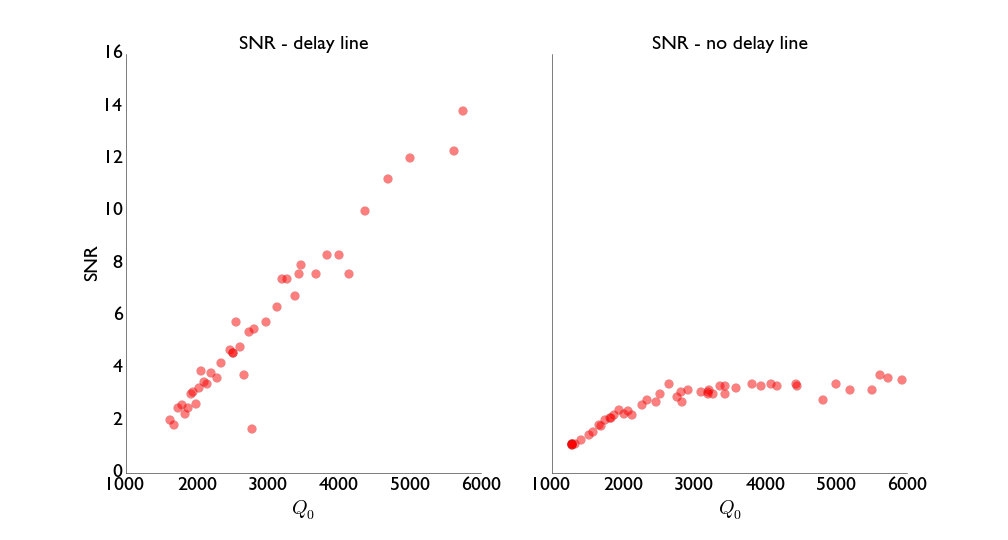
\includegraphics[width=\textwidth]{figs/summary_plots}
\caption{}
\label{fig:summary_plots}
\end{figure}

\section{Discussion}

We see in this prototype that with a very low Q cavity one can enhance the Q by a factor of more than a thousand, and see a signal to noise improvement of a factor of 10. This is extremely encouraging as a proof of principle, and shows that one can get to Q's comparable with the axion linewidth with the simple techniqure of active feedback. The main sources of systematic noise would come from gain instability in the circuit; in this experiment no noise additional to that expected was observed (or tested). This will increase the scan rate of microwave cavity experiments roughly by a factor of 3 and is simpler than research currently under way to improve the Q by making superconducting films on the walls of copper cavities. The active feedback technique becomes increasingly important for high-frequency axion experiments, as the passive limit for the Q scales as $f^{-1/3}$.

Delay lines with time delays longer than a few microseconds are difficult to make with analog technology; at 1 GHz and Q's of 100,000, we would need a delay of ten microseconds. Digital delay lines using FPGAs would be the natural way to implement the necessary delays.

%% Values of $M$ have been reported as high as $10^4$ yielding $Q$s of $7\times10^7$ in active feedback resonators~\cite{:/content/aip/journal/rsi/84/8/10.1063/1.4817537} used for other purposes, but that were operated at frequencies that could be relevant to dark matter axion searches.
%% This would suggest existing experiments could increase their SNR by several orders of magnitude by implementing active feedback.

The ADMX experiment is within an order of magnitude of the sensitivity necessary to be sensitive to pessimistically coupled axion dark matter.  The addition of active feedback, along with other planned upgrades, should allow it to to be sensitive to pessimistically coupled axion dark matter even in models where axions constitute a very small fraction of the dark matter.  The use of active feedback will also allow future experiments to operate at higher frequencies, where previous microwave cavity experiments have not had the sensitivity necessary to detect axion dark matter with a reasonable scan speed.

This work was supported in part by the U.S. Department of Energy under contract DE-SC0009800. A.M. would like to thank Ben Brubaker for helpful discussions.

\bibliography{2015_ouroboros}

\end{document}  
